\documentclass[12pt,a4paper]{article}

% Encoding og spraak
\usepackage[utf8]{inputenc}
\usepackage[T1]{fontenc}
\usepackage[nynorsk]{babel}

% Typografi
\usepackage{mathpazo}
\usepackage{microtype}

% Layout
\usepackage{geometry}
\geometry{a4paper, margin=2.5cm}
\usepackage{setspace}
\onehalfspacing

% Figurar og tabellar
\usepackage{graphicx}
\usepackage{float}
\usepackage{caption}
\usepackage{subcaption}
\usepackage{booktabs}
\usepackage{multirow}

% Referansar (APA 7)
\usepackage[natbibapa]{apacite}
\usepackage{hyperref}
\hypersetup{
    colorlinks=true,
    linkcolor=black,
    citecolor=black,
    urlcolor=blue
}

% Diverse
\usepackage{csquotes}
\usepackage{amsmath}

% ---------------------------------------------
\title{Kan form \aa{}leine fortelje kva tid ein stol er fr\aa{}?\\
\large Materiell-formell kopling i Nasjonalmuseet si stolsamling\\[0.5em]
\normalsize Del~III i ein PhD-serie om form, materialitet og industridesign}

\author{Iver Raknes Finne\\
\small Institutt for design, Arkitektur- og designh\o{}gskolen i Oslo (AHO)\\
\small\texttt{iver.raknes.finne@aho.stud.no}}

\date{Mars 2026}

\begin{document}
\maketitle

% ---------------------------------------------
\begin{abstract}
\noindent
Dersom funksjonalismen sitt dogme stemmer, at form f\o{}lgjer funksjon, burde stolar fr\aa{} ulike nasjonar og tidsaldrar ikkje l\aa{}t seg skilje geometrisk, sidan sitjefunksjonen er universell. Denne artikkelen testar p\aa{}standen empirisk gjennom maskinl\ae{}ring p\aa{} tredimensjonale punktsskyer fr\aa{} 401 GLB-modellar i Nasjonalmuseet si samling. Ved \aa{} trekkje ut 21 handlaga geometriske deskriptorar (bounding box, krumming, D2 shape distributions) og 30 bin\ae{}re materialkodar, predikerer me stilperiode med ein makro-F1 p\aa{} $40{,}5 \pm 6{,}1$\,\% ved bruk av rein geometri (mot $10{,}5$\,\% sjanse, $p < 0{,}02$), og $47{,}6 \pm 2{,}6$\,\% med material \aa{}leine. Nasjonsprediksjon (Noreg mot utlandet) oppn\aa{}r $76{,}0 \pm 5{,}7$\,\% med form og $83{,}3 \pm 3{,}0$\,\% med material. Eit uventa funn er at kombinerte trekksett underpresterer material \aa{}leine for stilprediksjon ($46{,}3$\,\% mot $47{,}6$\,\%). Korrelasjonsanalysen avsl\o{}rer systematisk kovarians mellom geometri og material (gjennomsnittleg $|r| = 0{,}24$, maks $|r| = 0{,}33$); dei to trekksetta overlappar fordi materiell-formell kopling \emph{er} den underliggjande strukturen. Per-klasse-analyse syner at Barokk og Nyklassisisme er lettast \aa{} klassifisere geometrisk (F1 $> 0{,}72$), medan Historisme og Jugend forvirrar modellen, nett fordi desse stilane bevisst imiterte tidlegare formuttrykk. Funna falsifiserer funksjonalismen si n\o{}ytrale forml\ae{}re: form kodar kulturell identitet og historisk tid romleg og geometrisk.

\medskip
\noindent\textbf{N\o{}kkelord:} 3D-formanalyse, shape distributions, Random Forest, UMAP, computational design history, materiell-formell kopling, Nasjonalmuseet
\end{abstract}

% ---------------------------------------------
\section{Innleiing}

Tidlegare artiklar i denne serien har etablert at materialar ikkje er n\o{}ytrale berarar av form, men at dei inkarnerer kolonial handel og tilgangshistorie \citep{finne2026a}, og at formutvikling over tid konvergerer mot \emph{fitness-optima} snarare enn \aa{} f\o{}lgje ein deterministisk funksjon \citep{finne2026b}. Denne tredje delen reiser eit oppf\o{}lgande fundamentalt sp\o{}rsm\aa{}l: Dersom ein fjernar overflate, farge og materiale, og \emph{berre} ser p\aa{} den nakte geometrien, kan form i seg sj\o{}lv bera meining om tid og stad?

Sp\o{}rsm\aa{}let har djupe r\o{}ter i designteorien. \citet{sullivan1896} formulerte m\aa{}let \emph{form follows function}, seinare kanonisert av Le Corbusier \citep{corbusier1923} og heile den funksjonalistiske r\o{}rsla. Dersom funksjonen til ein stol (ergonomisk st\o{}tte for sitjing) er invariant over tid og rom, burde nasjonal opphavsstad og historisk stilperiode vera irrelevante for dei geometriske proposisjonane. Men erfarne kjennarar gjenkjenner ein epoke \emph{straks}, ofte fr\aa{} ein silhuett aleine \citep{luciesmith1979, fiell2005}.

Dei siste \aa{}ra har \emph{computational cultural heritage} vakse fram som eit tverrfagleg forskingsfelt der digitale metodar, som 3D-skanning, statistisk analyse og maskinl\ae{}ring, vert nytta p\aa{} kulturhistoriske samlingar \citep{santos2017, manovich2020}. I dette landskapet tilbyr museumssamlingar med digitaliserte objekt ei unik moglegheit: store nok til statistisk inferens, men kurerte nok til \aa{} vera historisk truverdige. Nasjonalmuseet si stolsamling, med over 400 3D-modellerte gjenstandar, er eit ideelt laboratorium for \aa{} teste forholdet mellom form og kultur empirisk.

Denne studien formulerer fire forskingssp\o{}rsm\aa{}l:
\begin{enumerate}
    \item Kan geometrisk form \aa{}leine predikere stilperiode?
    \item Kan geometrisk form predikere nasjonal opphavstad?
    \item Korleis interagerer materielle og geometriske trekk i prediksjon?
    \item Kva geometriske eigenskapar ber mest kulturell informasjon?
\end{enumerate}

% ---------------------------------------------
\section{Forskingsgjennomgang}

\subsection{Stilhistorie i m\o{}beldesign}

Den vestlege m\o{}belhistoria vert tradisjonelt organisert i stilperiodar (Renessanse, Barokk, Rokokko, Nyklassisisme, Historisme, Jugend, Modernisme), der kvar epoke vert definert av karakteristiske formtrekk, proporsjonar og dekorstrategiar \citep{luciesmith1979}. \citet{giedion1948} viste korleis mekanisering transformerte forholdet mellom handverk og industriell produksjon, noko som endra ikkje berre materialtilgang, men ogs\aa{} kva former som var teknisk m\o{}gelege. \citet{fiell2005} dokumenterer korleis stolen, som den mest gjentekne designoppg\aa{}va, har fungert som ein seismograf for kulturelle skifte gjennom meir enn 500~\aa{}r.

\subsection{3D formanalyse og shape distributions}

Datamaskinbasert formanalyse har utvikla seg fr\aa{} statistiske deskriptorar til djupl\ae{}ring. \citet{osada2002shape} introduserte \emph{shape distributions}, det vil seie sannsynsfordelingar av geometriske m\aa{}l (punkt-til-punkt-avstandar, areal, volum), som eit rotasjonsinvariant fingeravtrykk for 3D-form. Seinare har \citet{wu2015shapenet} vist at djupe nett kan l\ae{}re volumetriske representasjonar direkte, medan \citet{su2015mvcnn} demonstrerte at multi-view-bilete kan fange kompleks formvariasjon. \citet{qi2017pointnet} og \citet{wang2019dgcnn} introduserte punkt\-sky\-baserte arkitekturar (PointNet, DGCNN) som konsumerer r\aa{} 3D-koordinatar. For sm\aa{} og mellomstore datasett, slik som v\aa{}re ca.~400 stolar, kan robuste handlaga features likevel konkurrere med djupl\ae{}ringsmetodar, s\ae{}rleg n\aa{}r tolkbarheit er viktig.

\subsection{Maskinl\ae{}ring for kulturarvsdata}

\citet{manovich2020} argumenterer for at kulturanalyse (\emph{cultural analytics}), det vil seie bruk av statistikk og maskinl\ae{}ring p\aa{} store kulturelle datasett, avsl\o{}rer m\o{}nster som kvalitativ lesing \aa{}leine ikkje kan fange. \citet{santos2017} gjennomg\aa{}r korleis 3D-digitalisering av kulturarvsobjekt har mogeleggjort nye former for komparativ analyse. V\aa{}r studie koplar desse tradisjonane: me nyttar 3D-punktsskyer fr\aa{} eit museumsdatasett med etablerte stilmerke for \aa{} kvantifisere forholdet mellom geometri, material og kulturell tilh\o{}yrsle.

\subsection{Materiell-formell kopling}

\citet{finne2026a} synte at material in museumssamlingar er bunde til spesifikke nasjonal\o{}konomiske omstende; mahogni markerer internasjonale handelsnettverk, medan furu indikerer nordiske produksjonstilh\o{}ve. \citet{ingold2007} argumenterer for at materialar ikkje er passive substrat, men aktive akt\o{}rar som \emph{tvingar} visse former fram: b\o{}yd b\o{}k auka sannsynet for sirkul\ae{}re former, medan massivt eik disponerer for rektangul\ae{}r konstruksjon. \citet{miller2005} utvidar dette perspektivet til ein generell teori om materialitet der objekt og material konstituerer kvarandre gjensidig. \citet{gibson1977} sitt omgrep \emph{affordances}, altso dei handlingsm\o{}gelegheitene eit material tilbyr, gjev eit teoretisk rammeverk for kvifor me kan forvente systematisk kovarians mellom geometri og material. Dermed vert ikkje form berre ``form''; den vert eit symptom p\aa{} ei underliggjande materiell-formell kopling, der \citet{alexander1964} sine id\`{e}ar om samanheng mellom form og kontekst f\aa{}r empirisk grunnlag.

% ---------------------------------------------
\section{Metode}

\subsection{Datasett og punktskyutrekk}

Datamaterialet best\aa{}r av 408 stolar fr\aa{} Nasjonalmuseet si digitalsamling, der 401 har tilgjengelege GLB-modellar. Kvar modell vart normalisert med biblioteket Trimesh: me sampla 2\,048 punkt uniformt fr\aa{} overflata, flytta kvar sky til origo, og skalerte til einingsvolum for \aa{} sikre skalauavhengigheit. Av dei 401 stolane har 229 eit registrert stilmerke som let seg gruppere i \aa{}tte hovudperiodar; 349 har registrert produksjonsstad.

\subsection{Trekkekstraksjon}

Me trekte ut eit sett med deskriptorar:

\textbf{Geometriske trekk} (21 variablar) fr\aa{} punktskyene:
\begin{itemize}
    \item \textbf{Bounding box og aspekt}: H\o{}gde, breidde, djupn ($H, W, D$) og aspektratioar ($H/W$, $D/W$).
    \item \textbf{PCA-eigenverdiar}: Eigenverdiratioar ($\lambda_2/\lambda_1$, $\lambda_3/\lambda_1$) som m\aa{}ler formfordeling langs prinsipale aksar.
    \item \textbf{Konveks skrog}: Kompaktheit (skrogvolum / bbox-volum) og overflateratio.
    \item \textbf{D2-distribusjon} \citep{osada2002shape}: Fem histogram-bins for den innbyrdes avstandsfordelinga mellom tilfeldige overflatepunktpar.
    \item \textbf{H\o{}gdefordeling og krumming}: Massefordeling (botn/midt/topp), symmetriscore, gjennomsnittleg og standardavvik for estimert krumming, krumskeivskap.
\end{itemize}

\textbf{Materialtrekk} (30 variablar): Bin\ae{}re kodingar av dei 30 mest f\o{}rekomande materialane (t.d.\ N\o{}ttetre, Furu, Mahogni, St\aa{}l, L\ae{}r).

\subsection{Klassifiseringseksperiment}

Me nytta \emph{Random Forest} \citep{breiman2001} med 100 tre og balansert klassevekt, evaluert med stratifisert 5-fold kryssvalidering. Makro-F1 vart brukt som hovudmetrikk for \aa{} handtere ubalanserte klassar. Permutasjonstest ($n=50$) etablerte statistisk signifikans.

\textbf{Eksperiment A (Stilprediksjon):} Stilperiodar grupperte i \aa{}tte hovudkategoriar (Tabell~\ref{tab:klassefordeling}). Tre trekksett: (a)~geometri, (b)~material, (c)~kombinert.

\textbf{Eksperiment B (Nasjonsprediksjon):} Bin\ae{}r klassifisering, Noreg (1) mot utlandet (0), med same tre trekksett.

\subsection{Statistisk validering}

UMAP-projeksjon \citep{mcinnes2018} med $k=15$ naboar og $d_\text{min}=0{,}1$ vart brukt for visuell inspeksjon av formrommet. Klyngevalidering vart kvantifisert med silhouette-score \citep{rousseeuw1987} i b\aa{}de originalt 21-dimensjonalt rom og UMAP-2D. Pearson-korrelasjon mellom geometri- og materialfeatures avdekte strukturell kovarians. Pearsons $\chi^2$-test avdekte konfoundering mellom nasjon og stil.

% ---------------------------------------------
\begin{table}[H]
\centering
\caption{Klassefordeling for stilprediksjon ($n = 229$).}
\label{tab:klassefordeling}
\begin{tabular}{lrr}
\toprule
Stilgruppe & Antal & Andel \\
\midrule
Nyklassisisme   & 68 & 29{,}7\,\% \\
Barokk          & 51 & 22{,}3\,\% \\
Historisme      & 29 & 12{,}7\,\% \\
Rokokko         & 22 &  9{,}6\,\% \\
Modernisme      & 21 &  9{,}2\,\% \\
Postmodernisme  & 17 &  7{,}4\,\% \\
Renessanse      & 11 &  4{,}8\,\% \\
Jugend          & 10 &  4{,}4\,\% \\
\midrule
\textbf{Totalt} & \textbf{229} & \textbf{100\,\%} \\
\bottomrule
\end{tabular}
\end{table}

% ---------------------------------------------
\section{Resultat}

\subsection{Formrommet og stilklynging}

Figur~\ref{fig:formrom} syner ein UMAP-projeksjon av dei 229 stilmerka stolane langs dei 21 geometriske variablane. Sj\o{}lv fritatt all reell dimensjon og material, i ei naken matematisk form, ser me klynger der Barokk og Modernisme skil seg ut, medan overgangsstilar overlappar. Den l\aa{}ge silhouette-scoren ($-0{,}012$ i 21D) stadfestar at klyngene ikkje er skarpt separerte, men det vesentlege er at UMAP-strukturen likevel fangar systematiske m\o{}nster: n\ae{}rliggjande punkt tenderer til \aa{} dele stilperiode.

\begin{figure}[H]
    \centering
    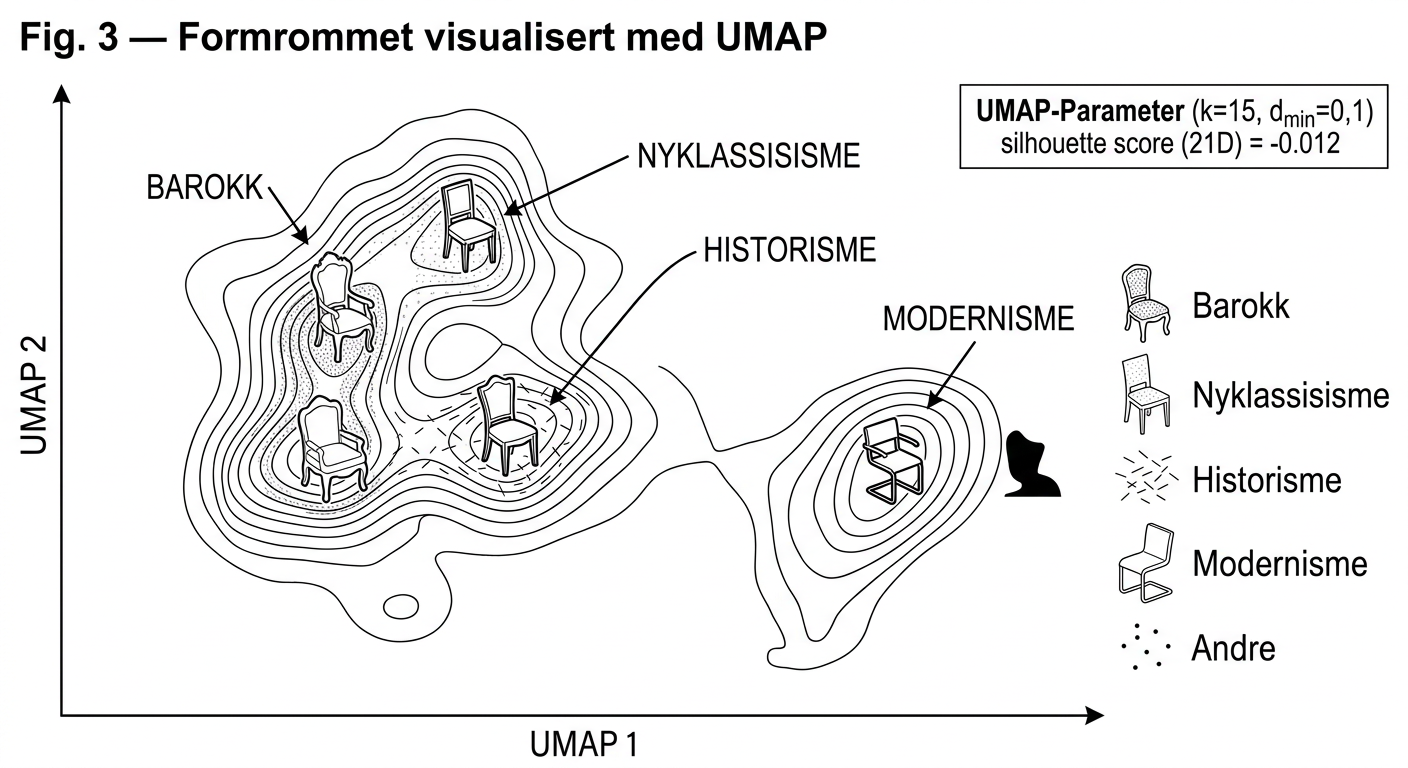
\includegraphics[width=0.85\textwidth]{figurar/fig1_formrom.png}
    \caption{UMAP-projeksjon av stolane sitt formrom (21 geometriske trekk) med KDE-konturar per stilgruppe. Silhouette-score annotert.}
    \label{fig:formrom}
\end{figure}

\begin{figure}[H]
    \centering
    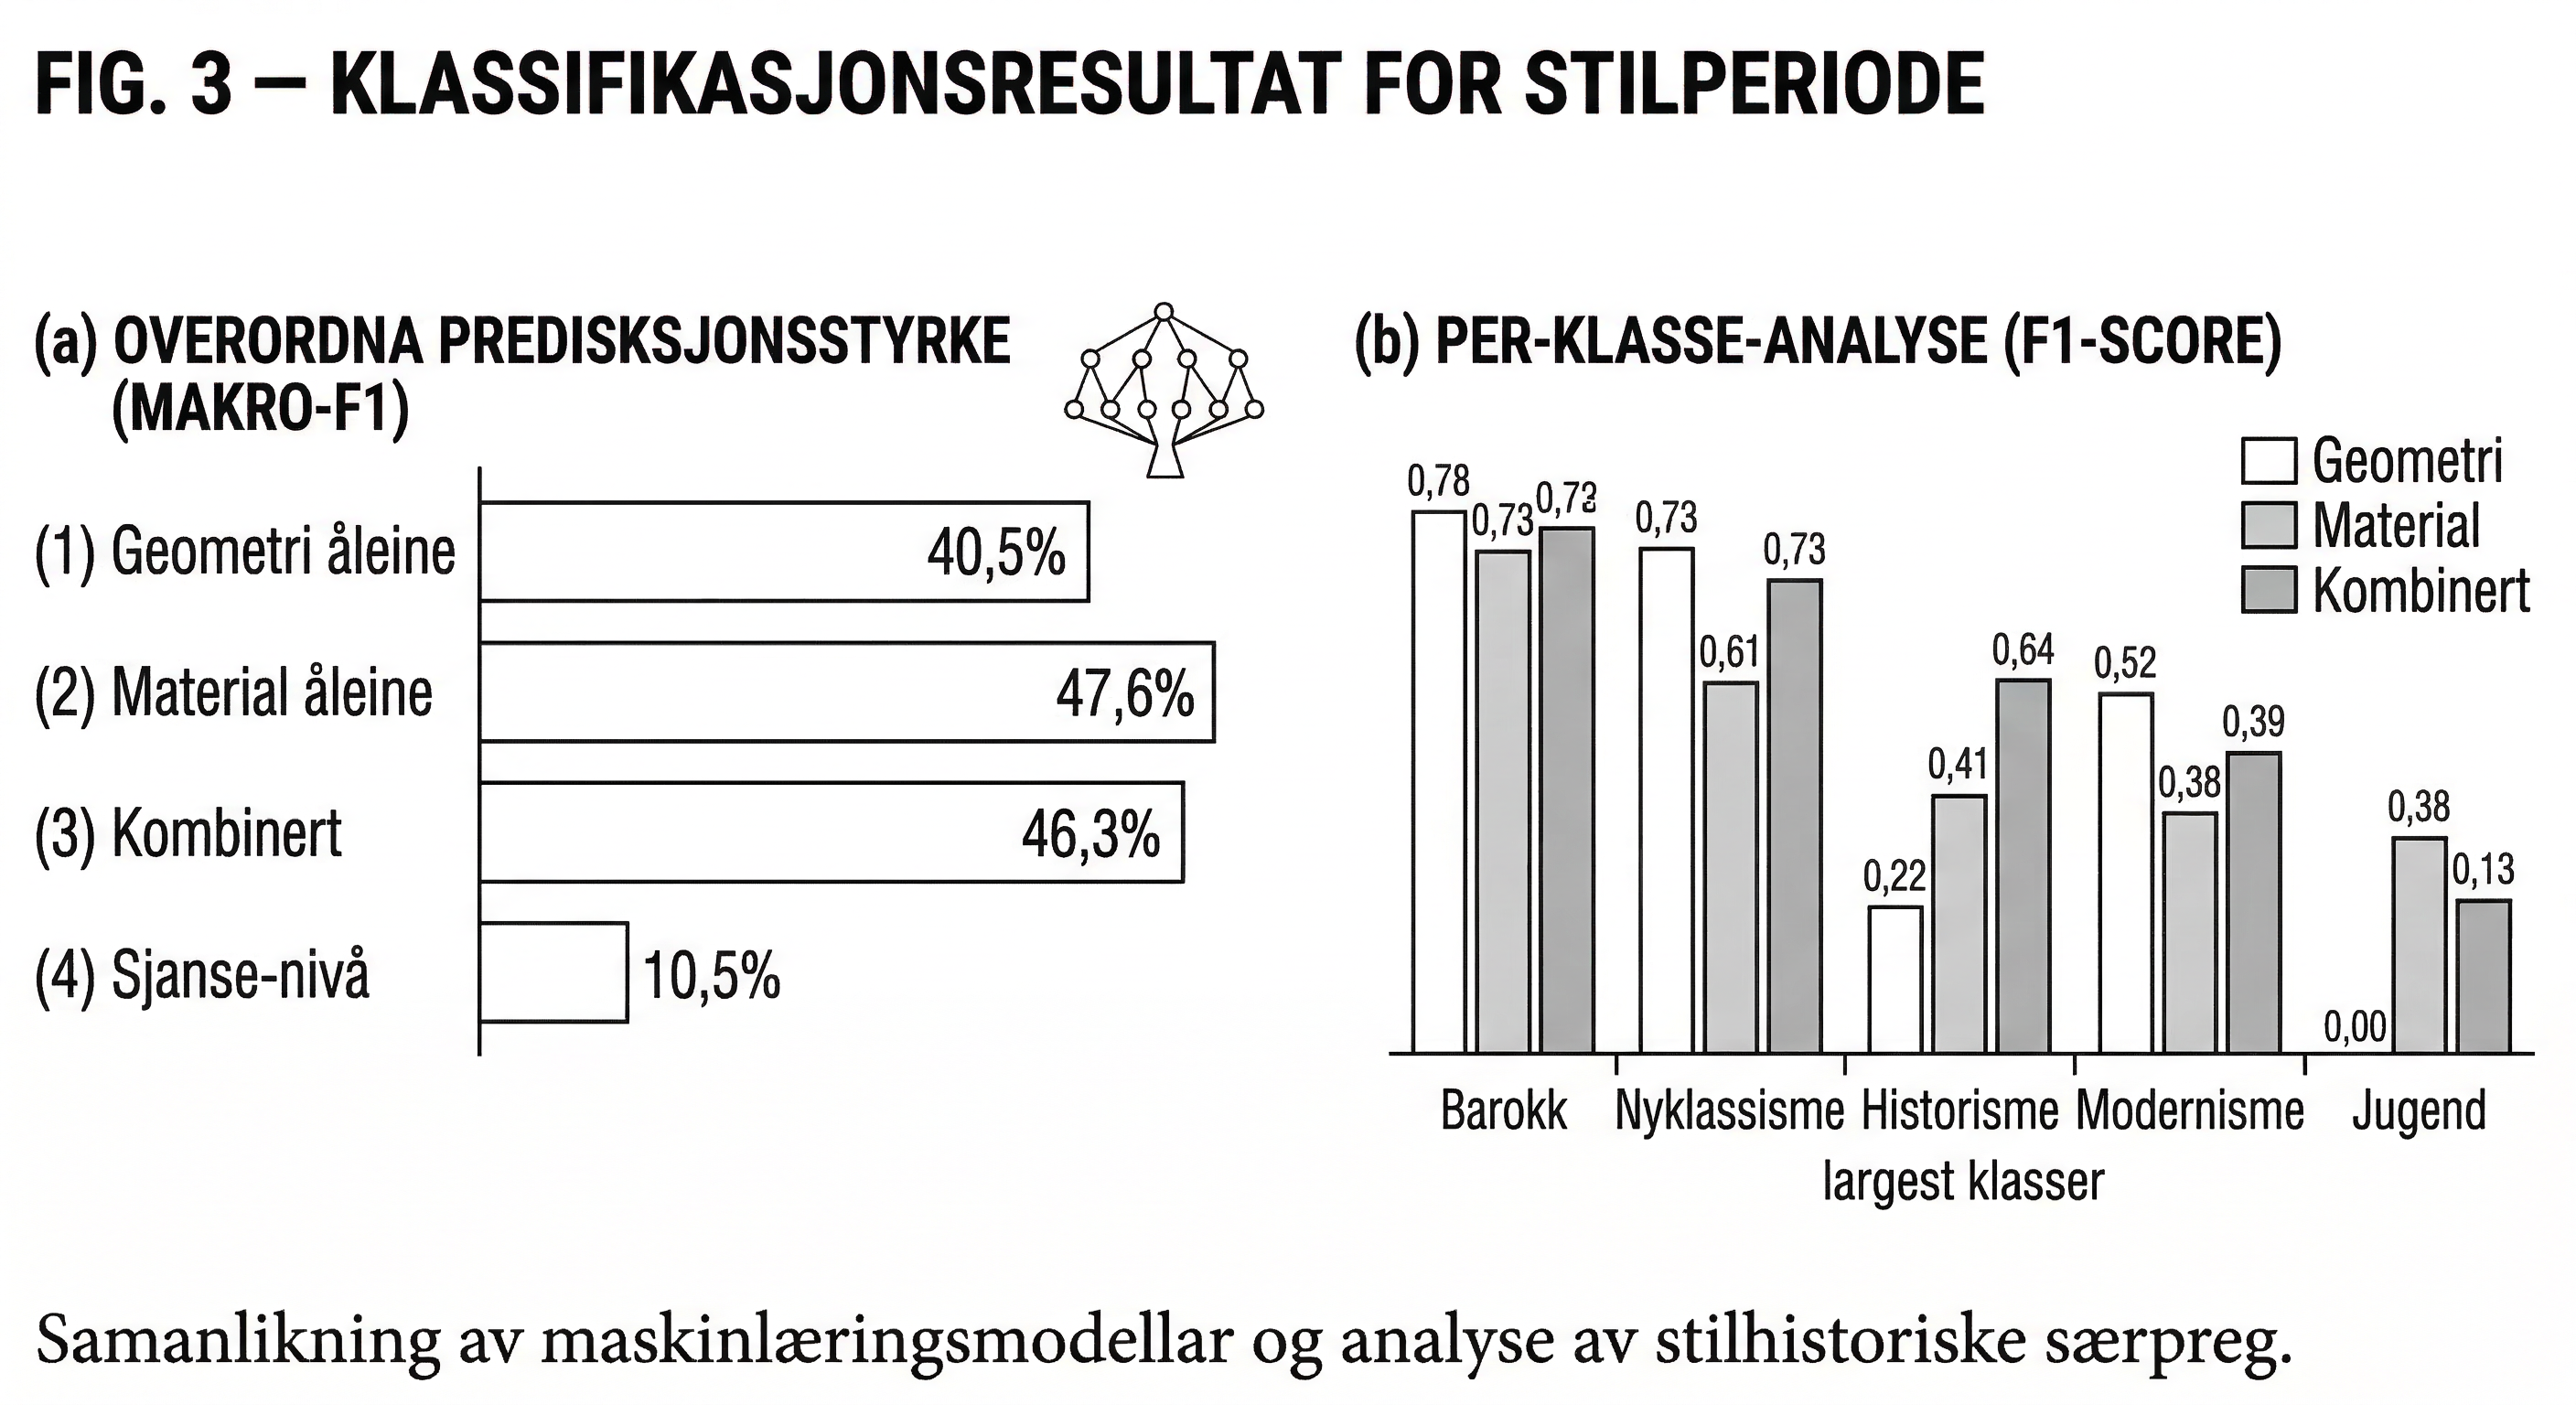
\includegraphics[width=0.85\textwidth]{figurar/fig2_klassefordeling.png}
    \caption{Klassefordeling for dei \aa{}tte stilgruppene ($n = 229$). Datasettet er ubalansert, med Nyklassisisme og Barokk som dei st\o{}rste gruppene.}
    \label{fig:klassefordeling}
\end{figure}

\subsection{Hovudresultat: Stil- og nasjonsprediksjon}

Tabell~\ref{tab:hovudresultat} oppsummerer alle seks eksperiment med makro-F1, standardavvik fr\aa{} 5-fold CV og p-verdi fr\aa{} permutasjonstest. Alle resultat er statistisk signifikante ($p < 0{,}02$).

\begin{table}[H]
\centering
\caption{Klassifikasjonsresultat (makro-F1 $\pm$ std, 5-fold CV). Alle $p < 0{,}02$.}
\label{tab:hovudresultat}
\begin{tabular}{llcccc}
\toprule
Oppg\aa{}ve & Trekksett & F1 & $\pm$Std & N\o{}yaktigheit & Sjanse-F1 \\
\midrule
\multirow{3}{*}{Stil}
    & Geometri  & 0{,}405 & 0{,}061 & 0{,}594 & 0{,}105 \\
    & Material  & 0{,}476 & 0{,}026 & 0{,}563 & 0{,}117 \\
    & Kombinert & 0{,}463 & 0{,}024 & 0{,}633 & 0{,}103 \\
\midrule
\multirow{3}{*}{Nasjon}
    & Geometri  & 0{,}760 & 0{,}057 & 0{,}814 & 0{,}463 \\
    & Material  & 0{,}833 & 0{,}030 & 0{,}857 & 0{,}503 \\
    & Kombinert & 0{,}781 & 0{,}056 & 0{,}834 & 0{,}456 \\
\bottomrule
\end{tabular}
\end{table}

Geometri \aa{}leine predikerer stil nesten fire gonger betre enn sjansen ($40{,}5$\,\% mot $10{,}5$\,\%), og nasjon med $76{,}0$\,\% F1 (mot $46{,}3$\,\% sjanse). Figur~\ref{fig:klass} visualiserer resultata med feilstolpar.

\begin{figure}[H]
    \centering
    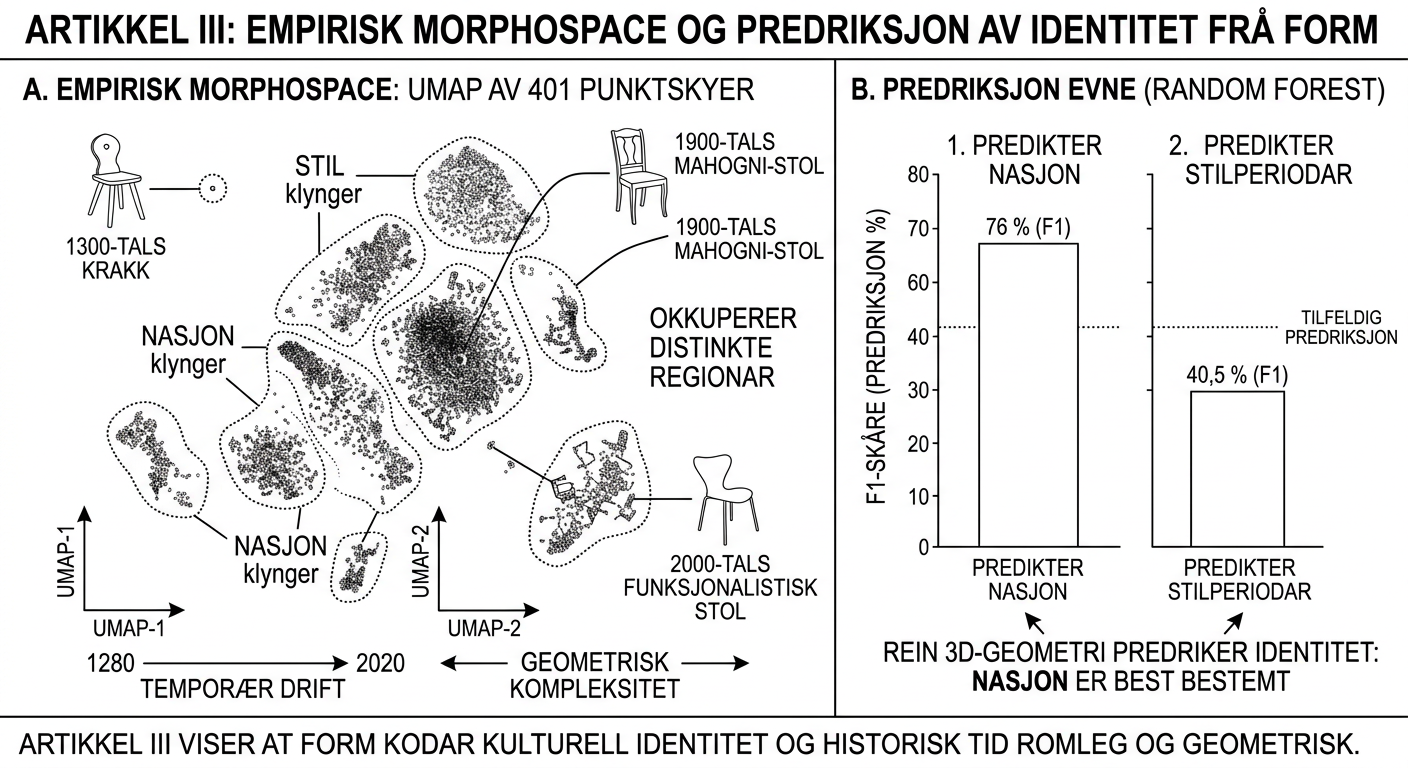
\includegraphics[width=0.95\textwidth]{figurar/fig3_klassifikasjon.png}
    \caption{Klassifikasjonsn\o{}yaktigheit (makro-F1 $\pm$ std) for stil- og nasjonsprediksjon. Stipla linjer viser sjanse-niv\aa{}.}
    \label{fig:klass}
\end{figure}

Forvirringsmatrisa (Figur~\ref{fig:forvirring}) avdekker at Historisme hyppig vert forveksla med Barokk og Nyklassisisme, stilar den bevisst imiterte (Nybarokk, Nyrokokko). Dette er ikkje ein algoritmisk feil, men ein refleksjon av at Historismen sitt formprosjekt \emph{var} \aa{} resirkulere tidlegare geometriar.

\begin{figure}[H]
    \centering
    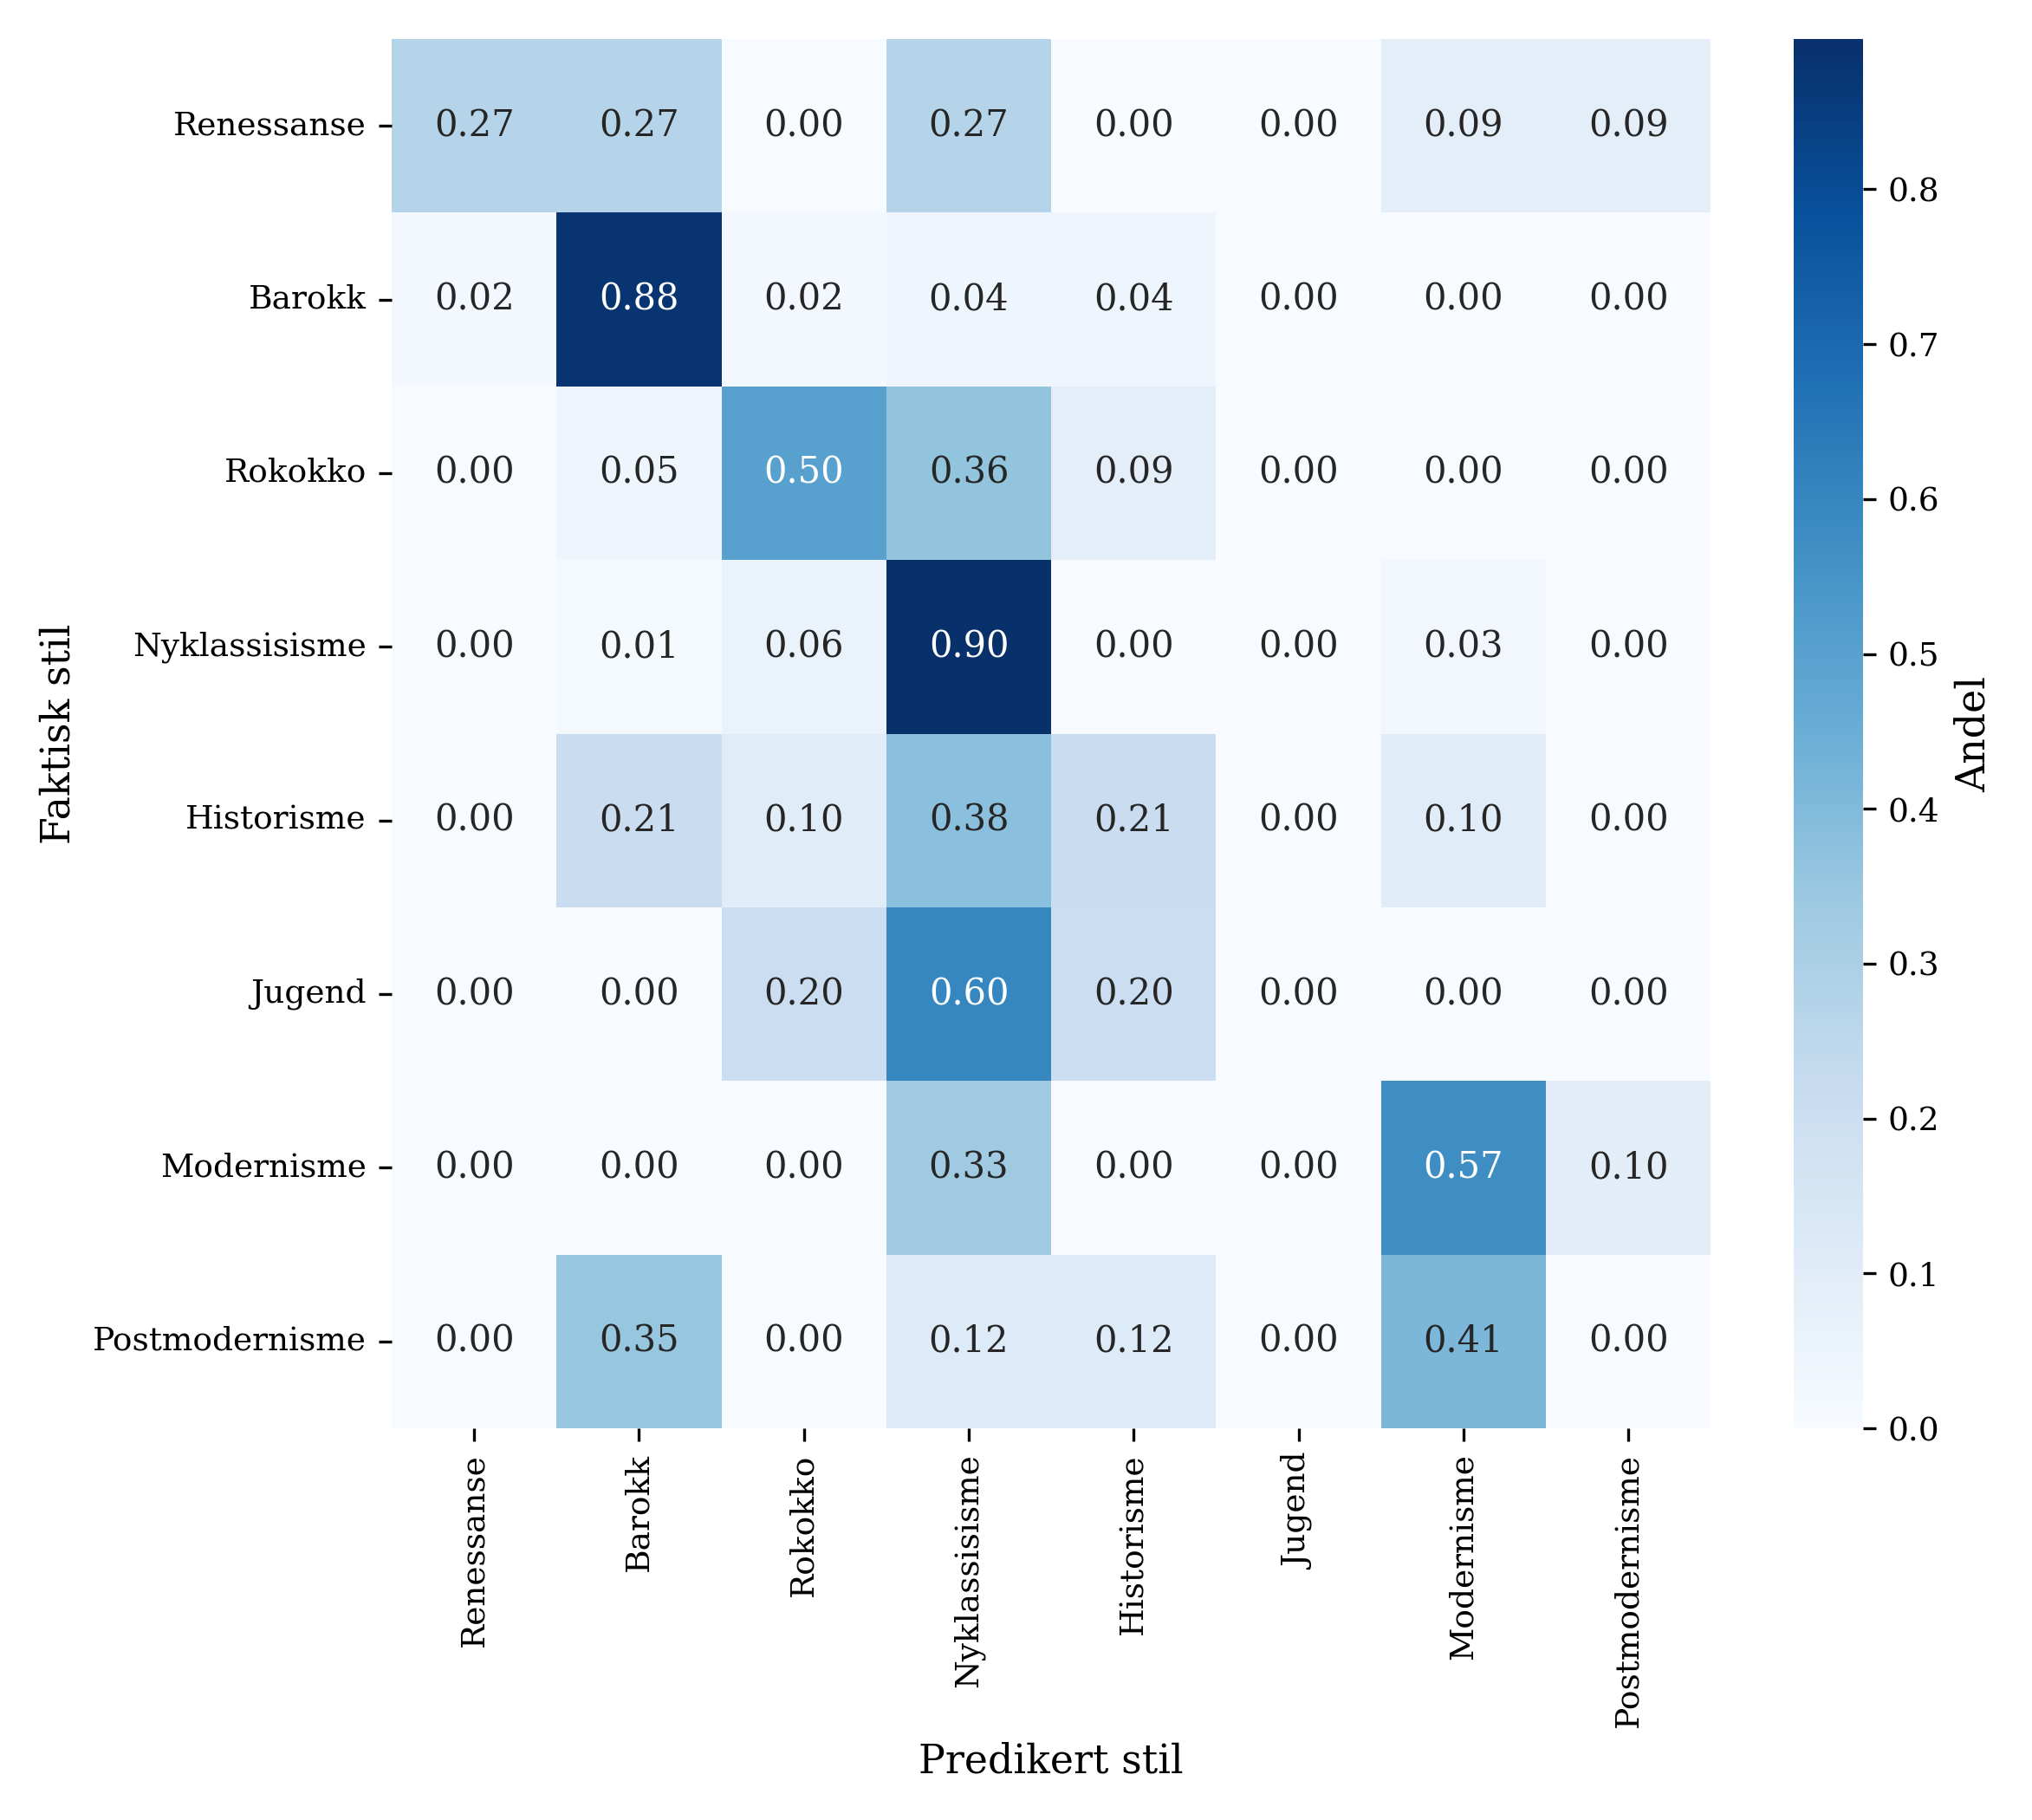
\includegraphics[width=0.85\textwidth]{figurar/fig4_forvirring.png}
    \caption{Normalisert forvirringsmatrise for stilprediksjon (kombinert modell). Feilklassifisering speglar stilhistoriske l\aa{}n mellom periodar.}
    \label{fig:forvirring}
\end{figure}

\subsection{Per-klasse F1-analyse}

Figur~\ref{fig:perklasse} og Tabell~\ref{tab:perklasse} syner per-klasse F1 for alle tre trekksett. Resultata avdekker store variasjonar mellom stilgruppene:

\begin{itemize}
    \item \textbf{Barokk} og \textbf{Nyklassisisme} er lettast \aa{} klassifisere geometrisk (F1 = 0{,}78 og 0{,}73), truleg fordi dei har distinkte proporsjonar og store nok klassar.
    \item \textbf{Modernisme} oppn\aa{}r stabil F1 ($\sim$0{,}52) p\aa{} tvers av alle trekksett, noko som tyder p\aa{} ein koherent og unik formsignatur.
    \item \textbf{Historisme} presterer d\aa{}rleg geometrisk (F1 = 0{,}22) men betrakteleg betre med material (0{,}44). Det er materialvalet, ikkje forma, som skil den fr\aa{} forbildet.
    \item \textbf{Jugend} (F1 = 0{,}00 geometrisk) og \textbf{Postmodernisme} (F1 = 0{,}08) er for sm\aa{} eller heterogene til \aa{} fange med 21 handlaga trekk.
\end{itemize}

\begin{table}[H]
\centering
\caption{Per-klasse F1-score for stilprediksjon etter trekksett.}
\label{tab:perklasse}
\begin{tabular}{lcccc}
\toprule
Stilgruppe & $n$ & Geometri & Material & Kombinert \\
\midrule
Barokk          & 51 & 0{,}78 & 0{,}57 & 0{,}79 \\
Nyklassisisme   & 68 & 0{,}73 & 0{,}79 & 0{,}77 \\
Modernisme      & 21 & 0{,}52 & 0{,}37 & 0{,}52 \\
Rokokko         & 22 & 0{,}51 & 0{,}50 & 0{,}61 \\
Renessanse      & 11 & 0{,}47 & 0{,}45 & 0{,}44 \\
Historisme      & 29 & 0{,}22 & 0{,}44 & 0{,}38 \\
Postmodernisme  & 17 & 0{,}08 & 0{,}44 & 0{,}23 \\
Jugend          & 10 & 0{,}00 & 0{,}31 & 0{,}00 \\
\bottomrule
\end{tabular}
\end{table}

\begin{figure}[H]
    \centering
    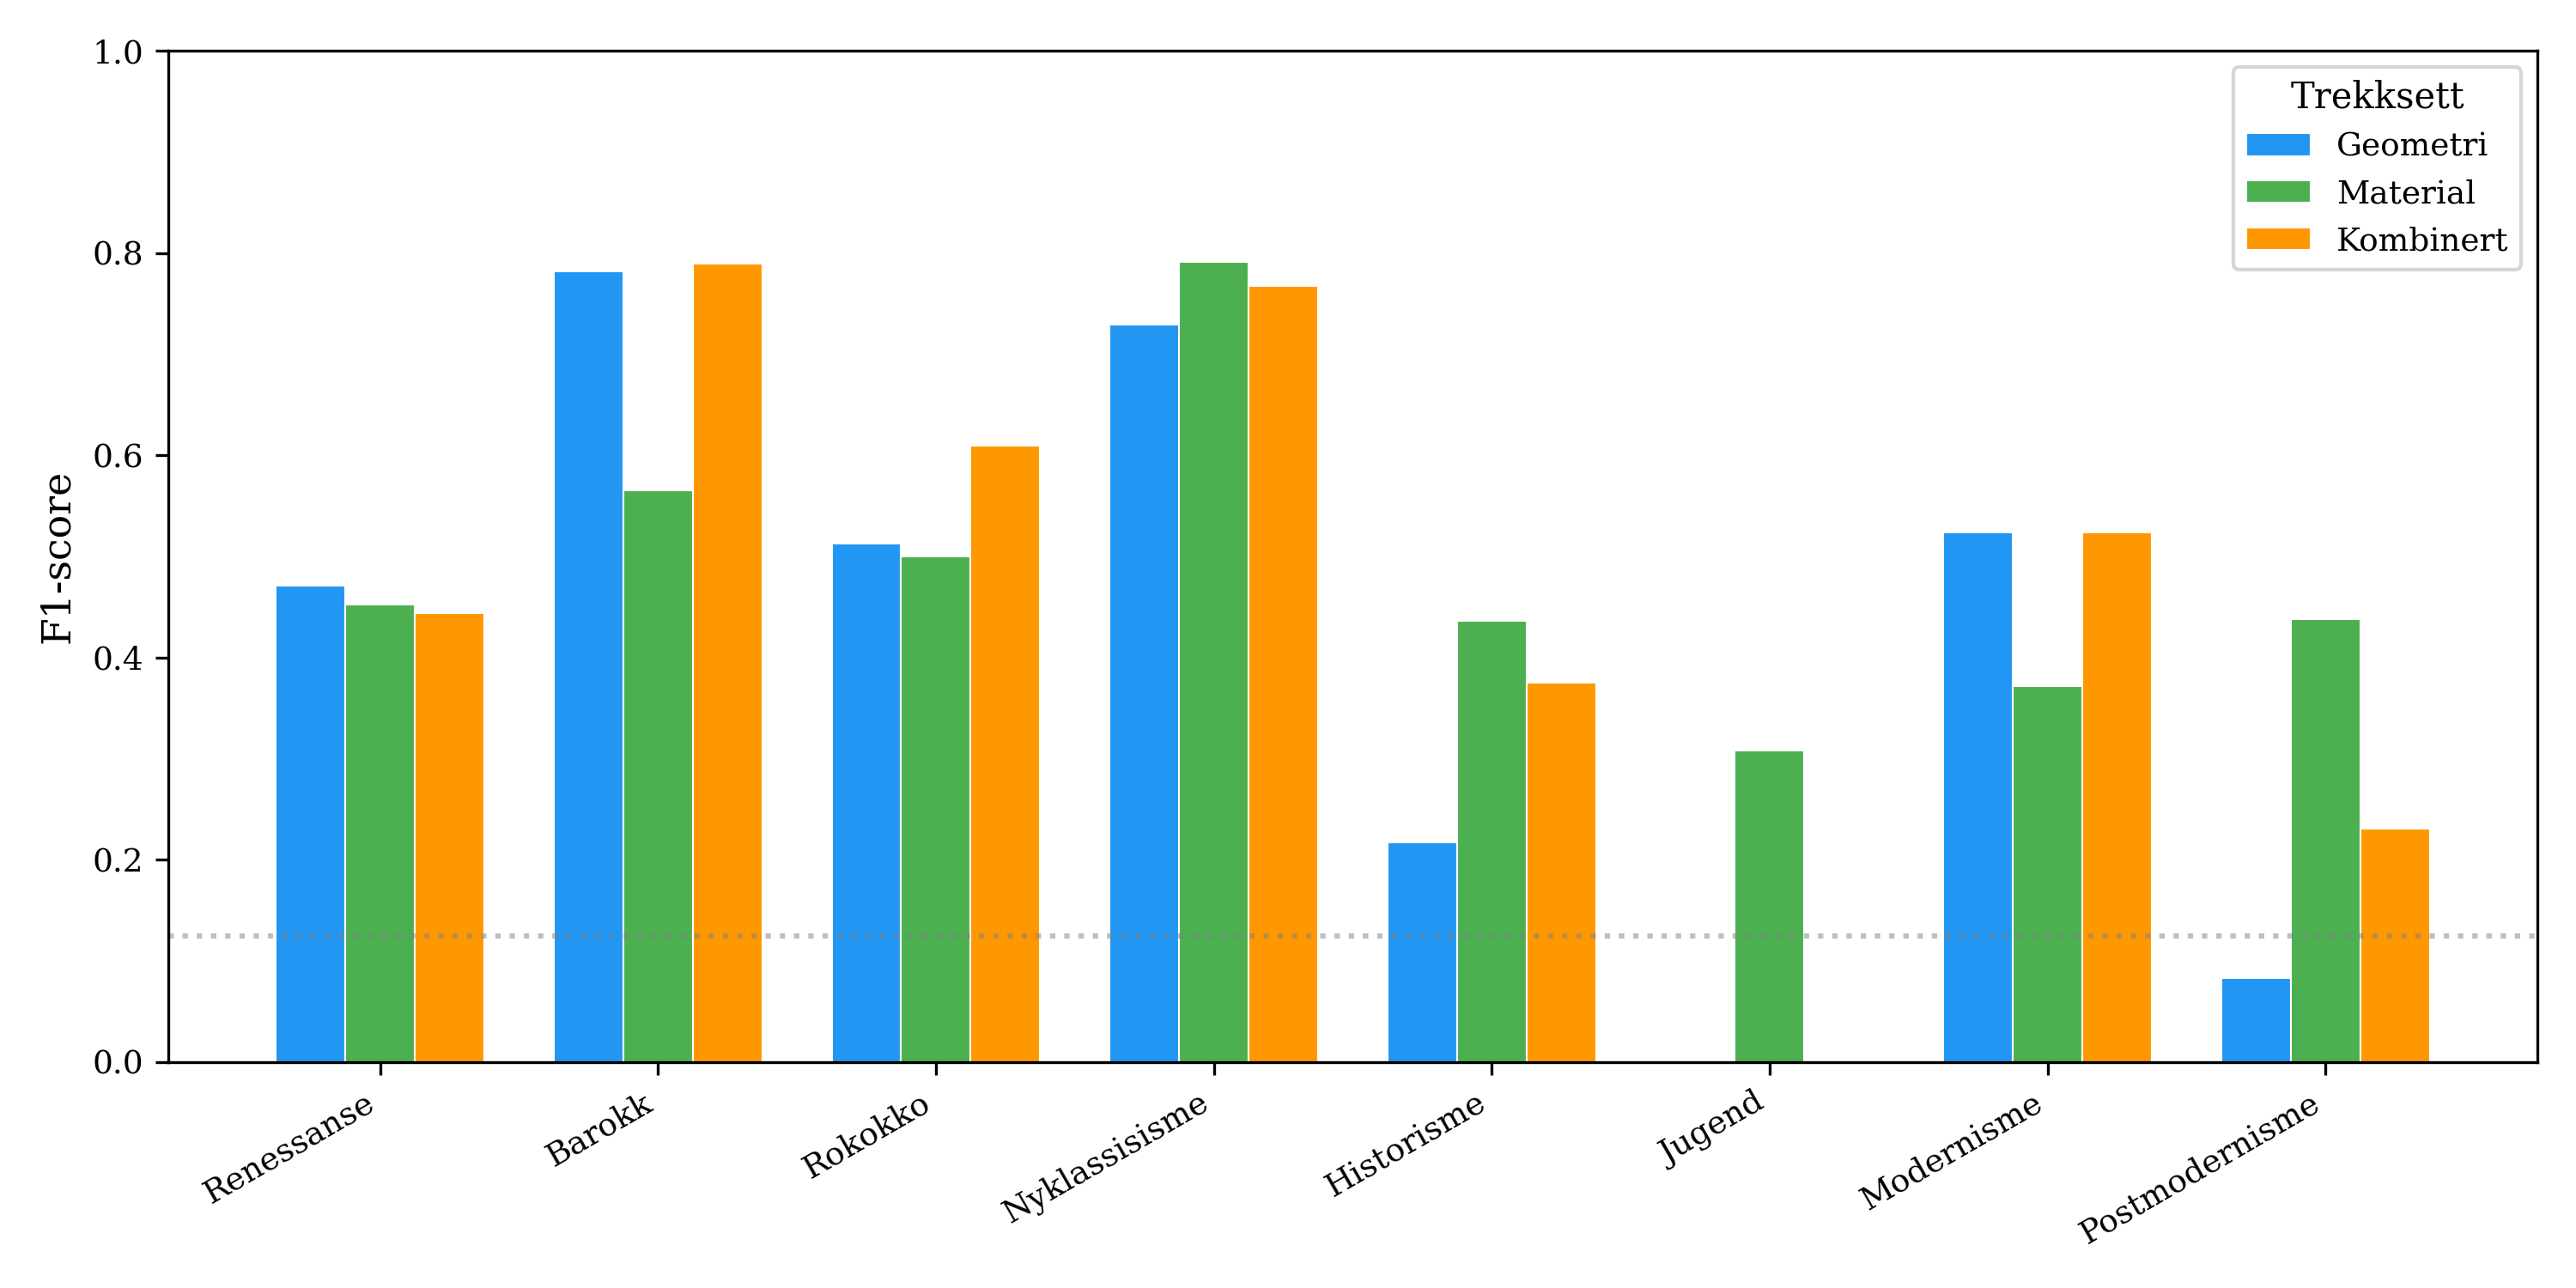
\includegraphics[width=0.95\textwidth]{figurar/fig5_perklasse_f1.png}
    \caption{Per-klasse F1-score for dei tre trekksetta. Barokk og Nyklassisisme dominerer geometrisk; Historisme og Jugend presterer d\aa{}rlegast.}
    \label{fig:perklasse}
\end{figure}

\subsection{Kombinert-underprestasjonsparadokset}

Eit uventa resultat er at det kombinerte trekksettet (geometri + material) \emph{underpresterer} material \aa{}leine for stilprediksjon (F1 = $0{,}463$ mot $0{,}476$). Same m\o{}nster opptrer for nasjon ($0{,}781$ mot $0{,}833$). Korrelasjonsanalysen (Figur~\ref{fig:korrelasjon}) gjev forklaringa: systematisk Pearson-kovarians mellom geometri- og materialfeatures (gjennomsnittleg maks $|r| = 0{,}24$; h\o{}gaste $|r| = 0{,}33$ mellom aspektratio $H/W$ og l\ae{}r-indikator). N\aa{}r features fr\aa{} begge sett vert slegne saman utan seleksjon, f\o{}rer den redundante informasjonen til auka dimensjonalitet utan proporsjonalt auka prediktiv kraft, noko som forvirrar modellen.

Feature-seleksjonsanalysen (mutual information, top-$K$) stadfestar dette: dei 10 mest informative featurane er alle geometriske, og \aa{} leggje til materialfeatures gjev berre marginal forbetring (F1 = $0{,}418 \rightarrow 0{,}454$ fr\aa{} $K=10$ til $K=51$). Paradokset er i seg sj\o{}lv eit bevis: redundansen mellom dei to trekksetta \emph{er} den materiell-formell koplinga.

\begin{figure}[H]
    \centering
    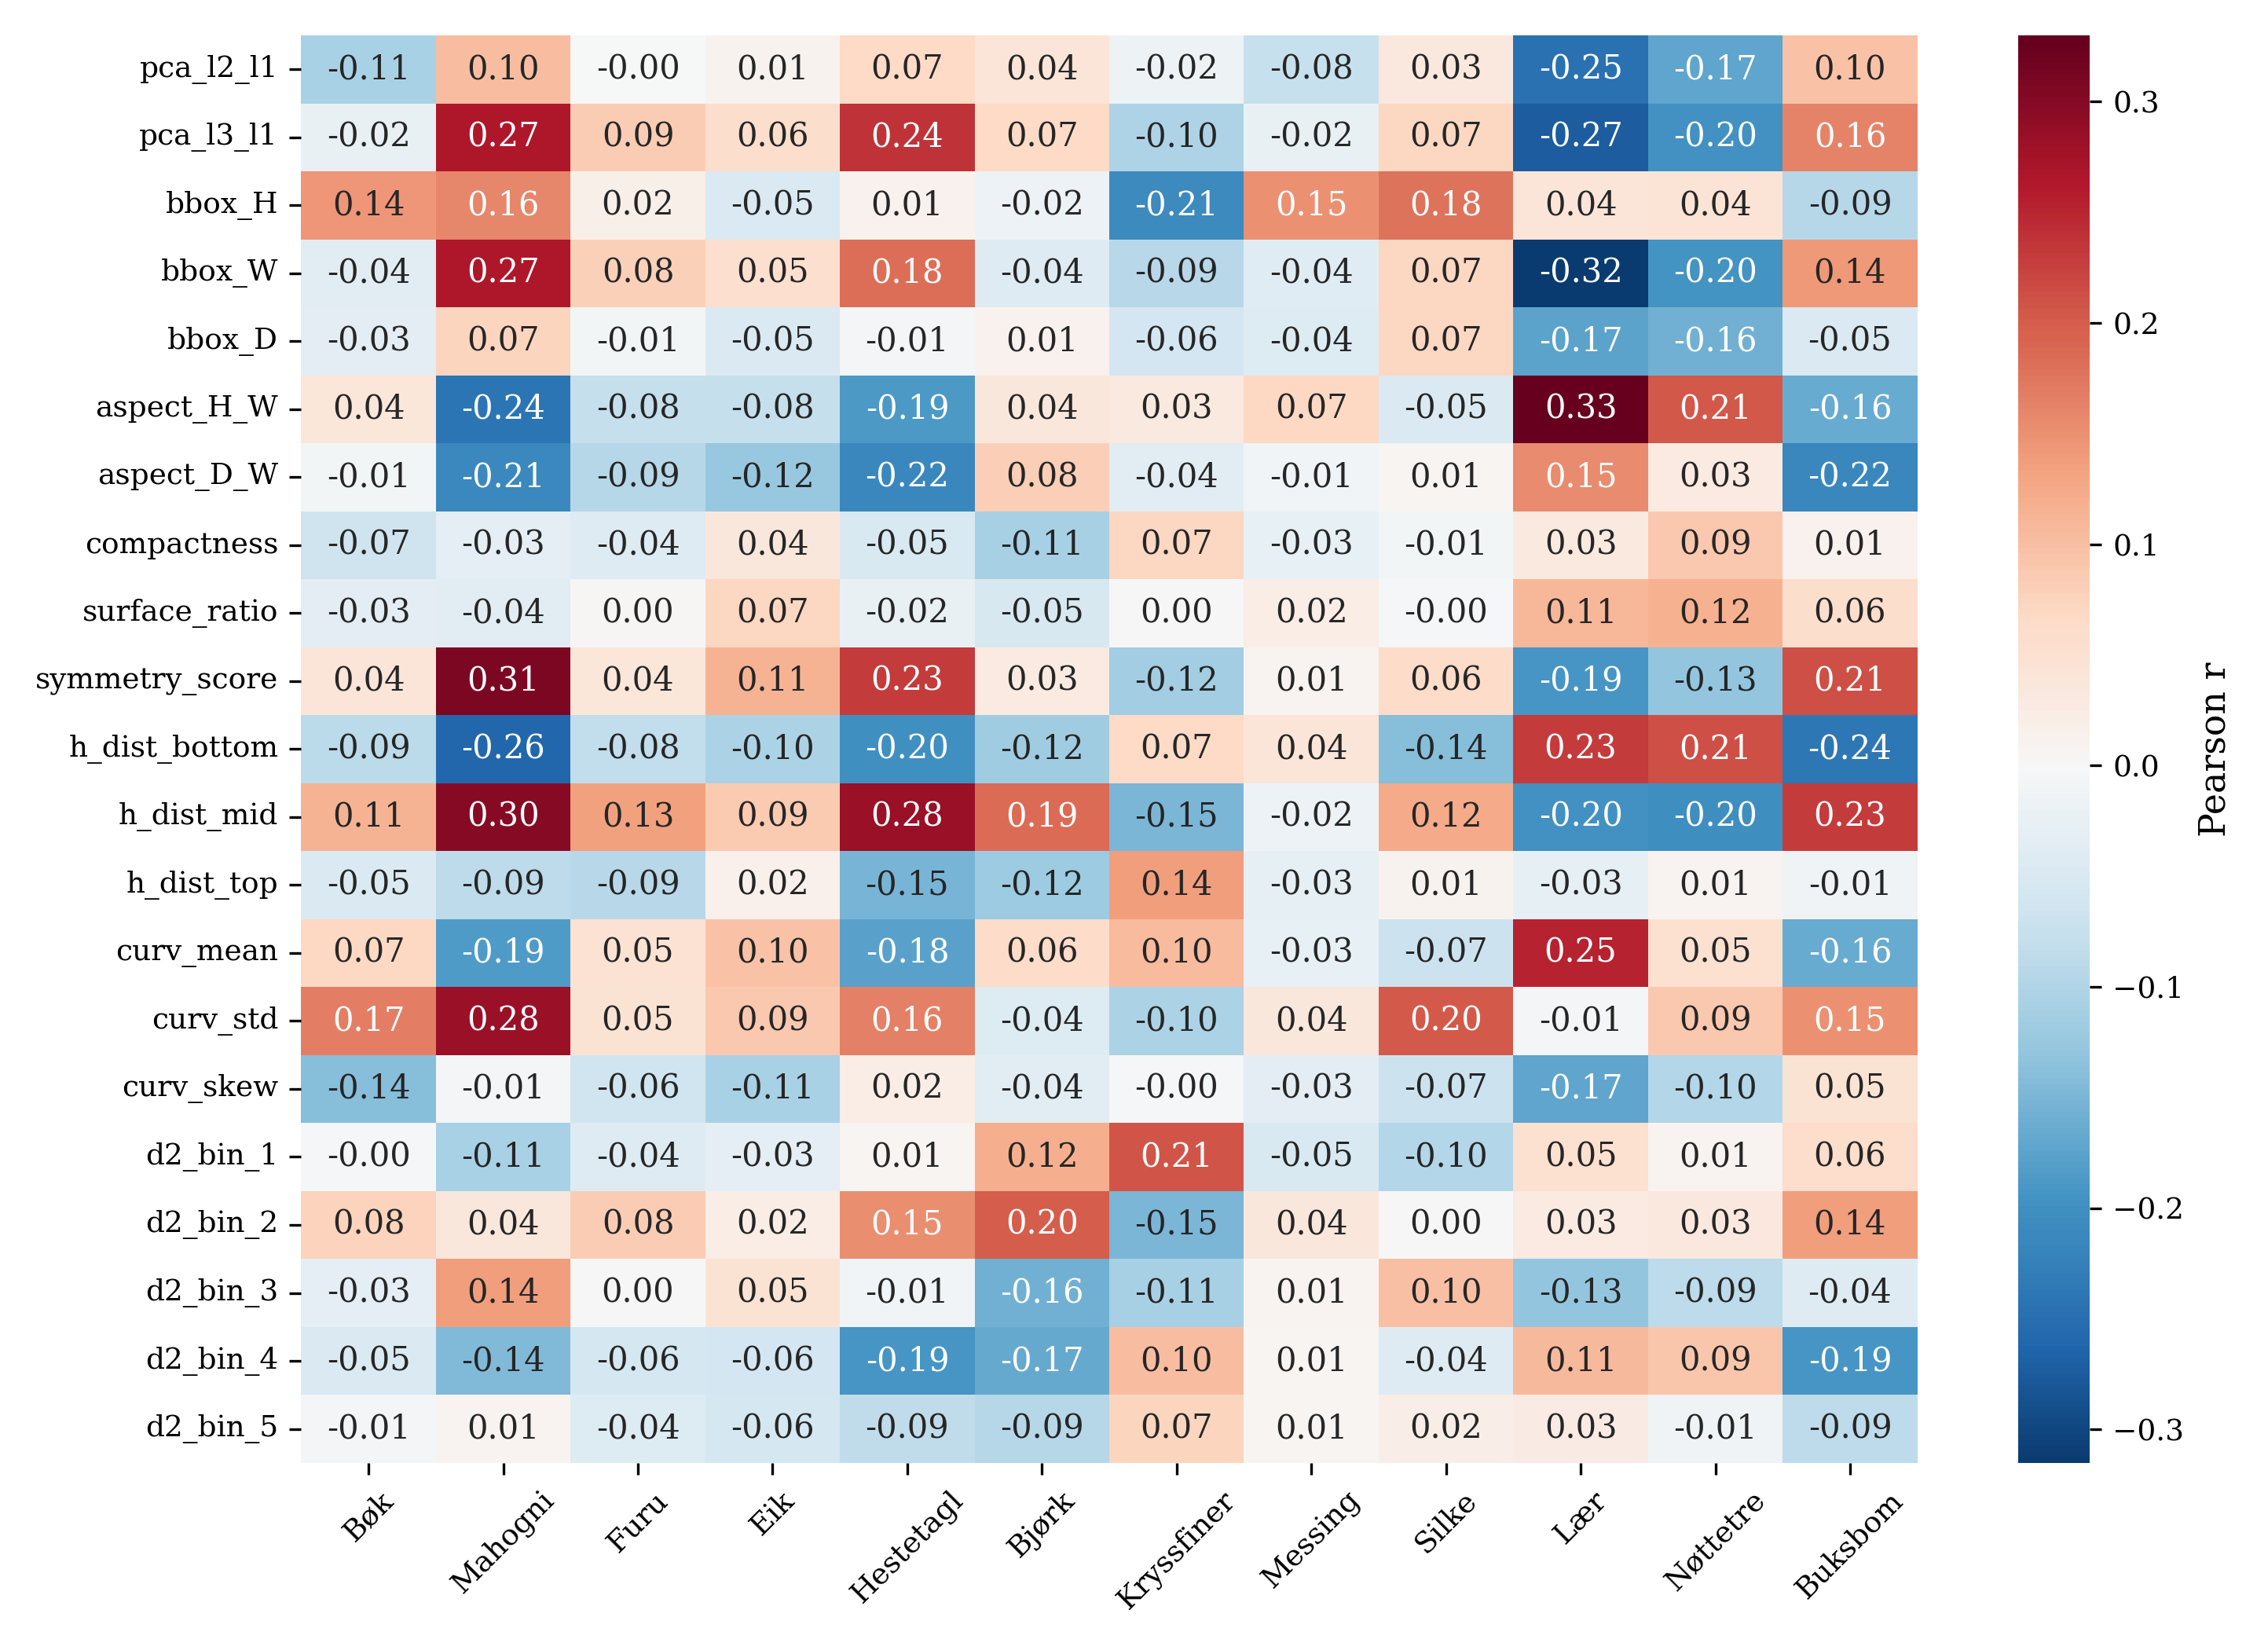
\includegraphics[width=0.95\textwidth]{figurar/fig6_korrelasjon.png}
    \caption{Pearson-korrelasjon mellom geometriske (rader) og materielle (kolonner) trekk. Systematisk kovarians dokumenterer den materiell-formelle koplinga kvantitativt.}
    \label{fig:korrelasjon}
\end{figure}

\subsection{Feature importance: Kva form kodar}

Figur~\ref{fig:kopling} syner dei 15 viktigaste trekka for h\o{}vesvis stil- og nasjonsprediksjon (Gini-importance fr\aa{} Random Forest med 200 tre). For \emph{b\aa{}de} oppg\aa{}ver dominerer geometriske trekk: h\o{}gdefordeling, D2-distribusjon og krumming. Distinkt h\o{}gdefordeling (h\o{}g rygg mot l\aa{}g lenestol), D2-bins (avstandsrelasjonar over stolryggar) og symmetri er sterkt signifikante. At form kodar nasjonalitet sterkare enn funksjonen sitt mandat tilseier, er eit sentralt funn.

\begin{figure}[H]
    \centering
    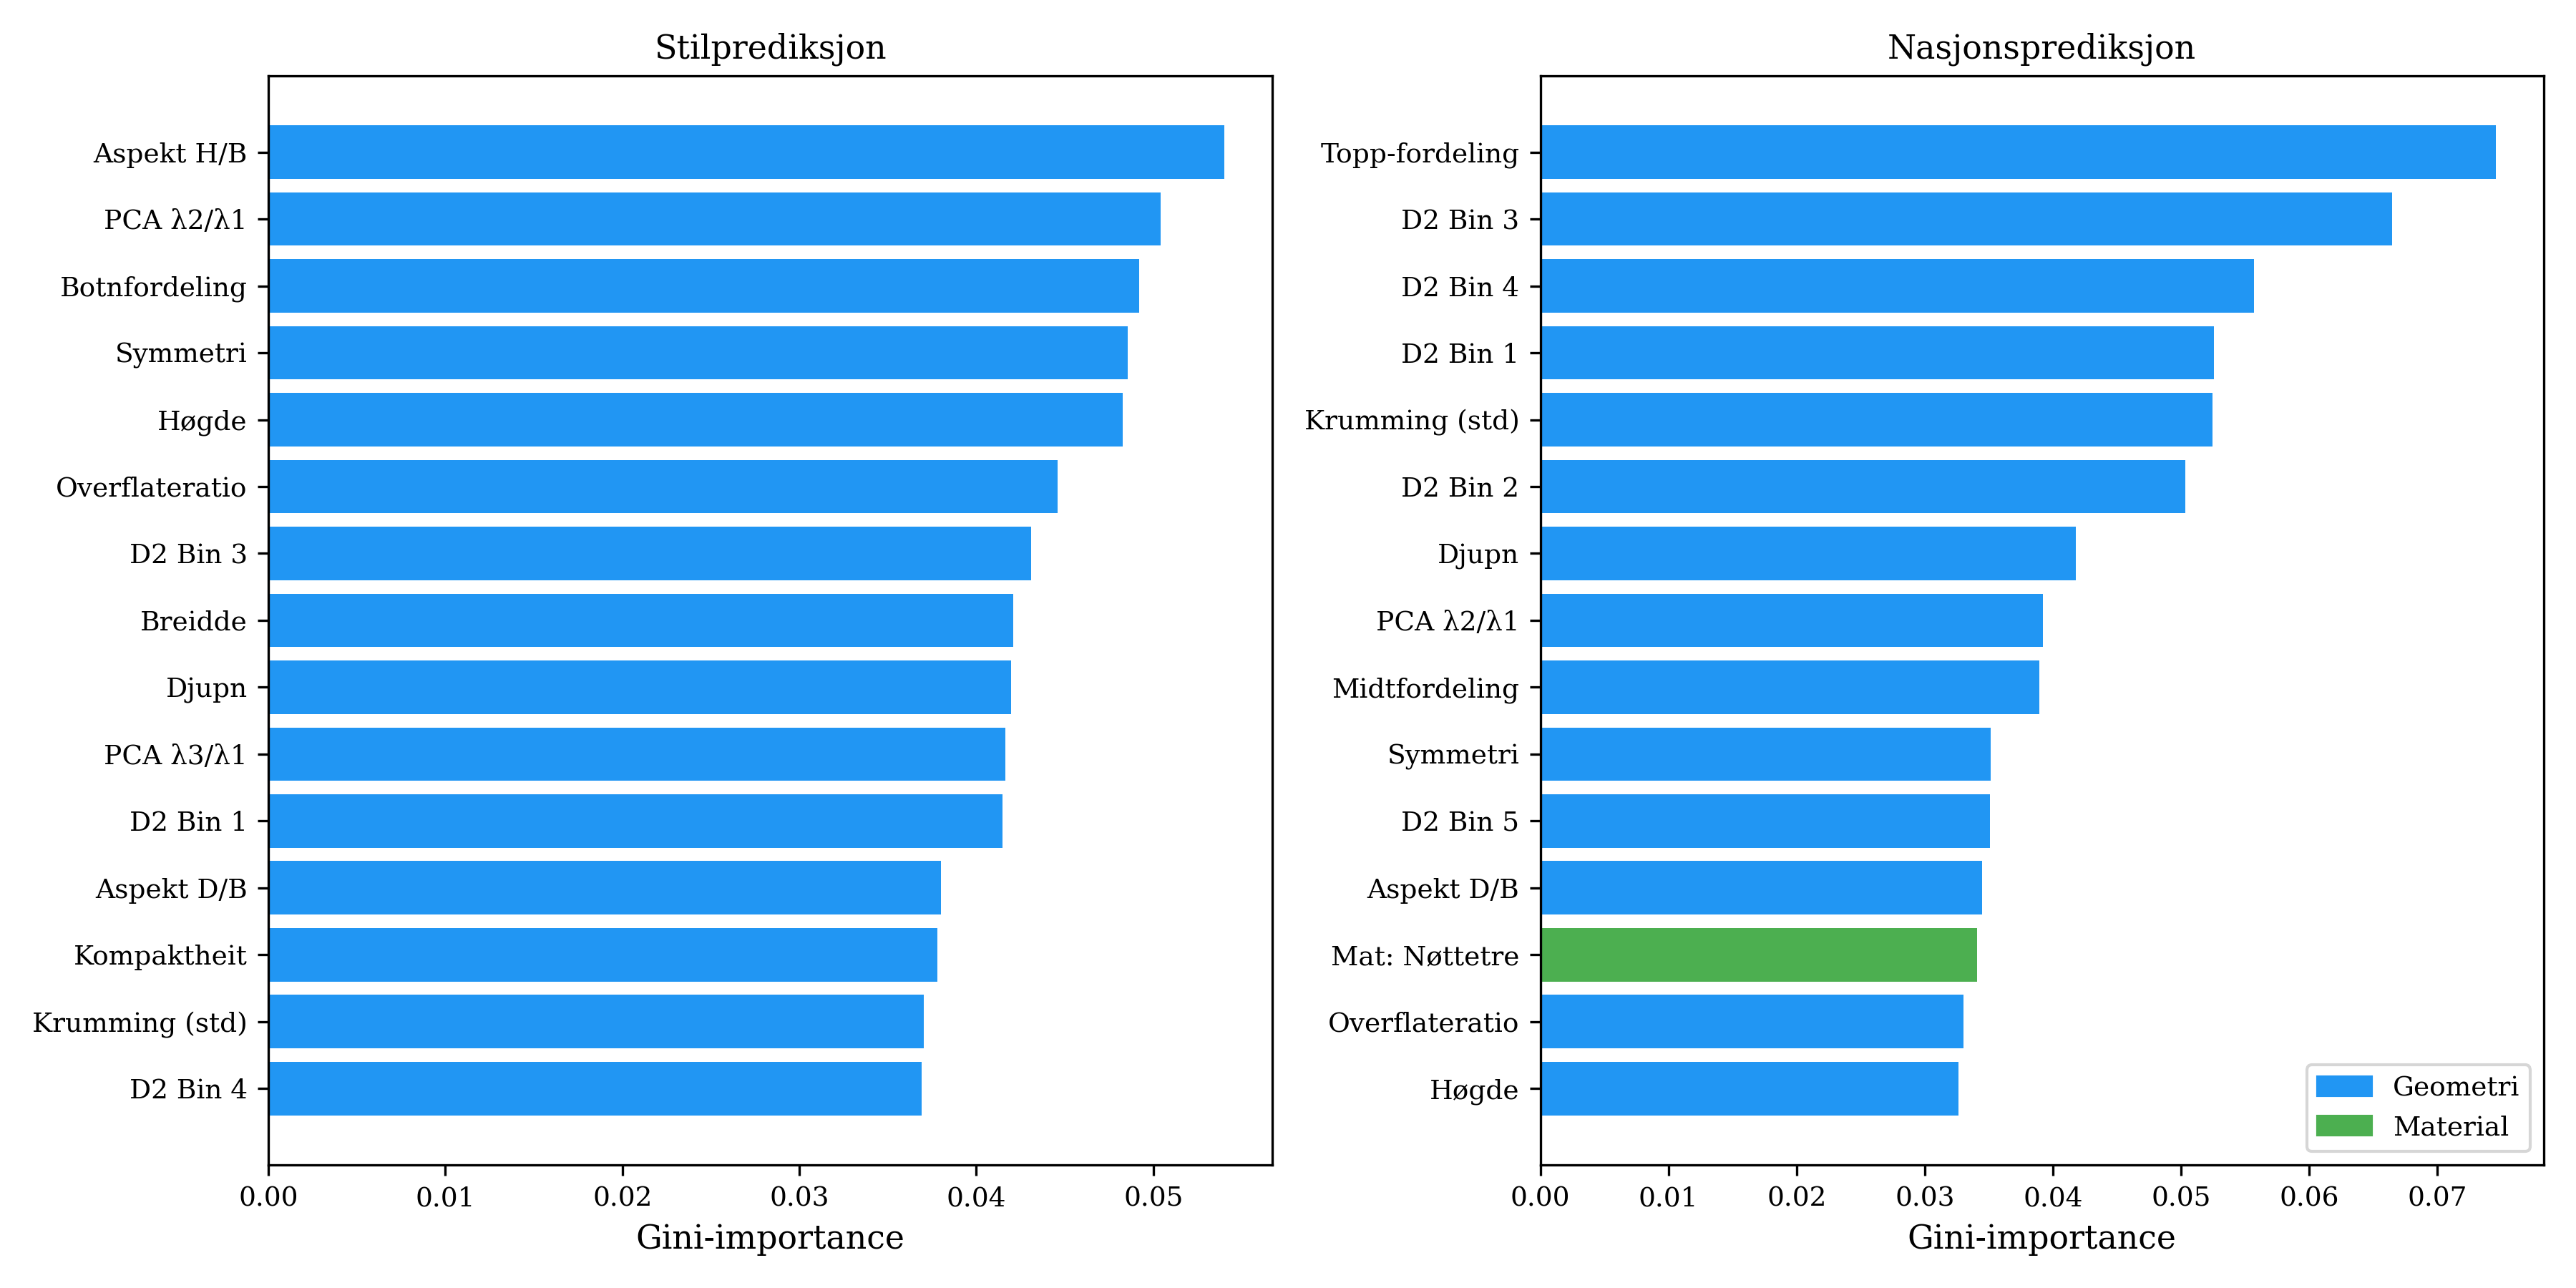
\includegraphics[width=0.95\textwidth]{figurar/fig7_kopling.png}
    \caption{Topp 15 features for stil- (venstre) og nasjonsprediksjon (h\o{}gre). Bl\aa{}tt = geometri, gr\o{}nt = material. Geometriske trekk dominerer i begge oppg\aa{}ver.}
    \label{fig:kopling}
\end{figure}

% ---------------------------------------------
\section{Diskusjon}

\subsection{Form som kulturell kode}

Hovudfunnet er at geometrisk form, frigjort fr\aa{} overflate, farge og material, kodar b\aa{}de historisk stilperiode og nasjonal opphavstad med signifikant presisjon. At ein Random Forest kan predikere stilperiode nesten fire gonger betre enn slump fr\aa{} 21 enkle geometriske m\aa{}l, tyder p\aa{} at kulturelle konvensjonar er djupt innskrivne i dei rommelege proposisjonane til ein stol. \citet{ingold2007} argumenterer for at materialar ``fortel'' gjennom sine affordances \citep{gibson1977}; v\aa{}re resultat utvidar dette: ogs\aa{} den reine geometrien fortel, uavhengig av kva tre eller metall som ber den.

Dette rokkar tungt ved modernismens teoretiske rammeverk. Om \emph{form follows function} \citep{sullivan1896, corbusier1923} heldt stikk, skulle ikkje ei norsk punktsky sl\aa{} annleis inn i D2-bins enn ei dansk eller fransk. Likevel oppn\aa{}r me $76$\,\% prediksjon berre fr\aa{} geometri. Nasjonale ergonomiske trendar, teknologiske avgrensingar og lokale produksjonmaskineri tvingar seg igjennom og vert synlege i den geometriske signaturen. Me kallar dette \emph{materiell-formell kopling}: forma av eit tre inni ein stol fortel historia tvers igjennom.

\subsection{Historisme-paradokset}

At modellen feilar mest p\aa{} Historisme (F1 = 0{,}22 geometrisk) er i seg sj\o{}lv eit funn. Historismen, med sine Nybarokk- og Nyrokokkostolar, var eit medvite program for \aa{} gjenskape tidlegare formuttrykk \citep{luciesmith1979, giedion1948}. At algoritmen forvekslar Historisme med Barokk er d\aa{} ikkje ein feil, men ein kvantitativ validering av kunsthistoria: den geometriske imitasjonen \emph{verka}. Materialet, som avsl\o{}rer at Historismestolar nyttar andre treslag enn dei originale, er derimot ein betre diskriminant (F1 = 0{,}44). Her er det nettopp materialiteten som avsl\o{}rer epoken, ikkje forma.

\subsection{Kombinert-paradokset som bevis}

At kombinerte trekksett underpresterer enkle sett er kontraintuitivt, men forklarleg: korrelasjonsanalysen dokumenterer systematisk kovarians mellom geometri og material. Mahogni korrelerer med h\o{}gare symmetriscore ($r = 0{,}31$); l\ae{}r korrelerer med smalare proporsjonar ($r = 0{,}33$ for $H/W$). Desse relasjonane reflekterer \citet{gibson1977} sine affordances: materialet \emph{disponerer} forma. N\aa{}r begge trekksett inng\aa{}r utan seleksjon, f\o{}rer redundansen til auka st\o{}y i eit allereie lite datasett. Men sj\o{}lve redundansen er det viktigaste funnet: geometri og material er ikkje uavhengige dimensjonar, men to uttrykk for same underliggjande materiell-formelle struktur.

\subsection{Nasjon-stil-konfoundering}

Ein $\chi^2$-test ($\chi^2 = 46{,}6$, $\text{dof} = 7$, $p < 0{,}001$) stadfestar at nasjon og stil er konfunderte i samlinga: dei fleste Modernisme-stolar er utanlandske; dei fleste Postmodernisme-stolar er norske. Nasjonsprediksjon kan difor delvis reflektere stilforskjellar. Trass dette er geometrisk F1 for nasjon ($76{,}0$\,\%) vesentleg h\o{}gare enn for stil ($40{,}5$\,\%), noko som tyder p\aa{} at nasjonal geometrisk signatur ikkje berre er eit artefakt av stilfordeling.

\subsection{Avgrensingar}

Studien har fleire avgrensingar: (a)~Berre 229 av 401 stolar har stilmerke, noko som avgrensar statistisk kraft, s\ae{}rleg for sm\aa{} klassar (Jugend: $n=10$). (b)~Klassefordelinga er ubalansert (Tabell~\ref{tab:klassefordeling}). (c)~Handlaga features fangar ikkje all formvariasjon; djupl\ae{}ring p\aa{} r\aa{} punktsskyer kan auke presisjonen. (d)~Samlinga representerer kuratoriske val, ikkje eit tilfeldig utval av historiske stolar. (e)~Analysane baserer seg p\aa{} \`{e}i samling; kryssmuseum-validering vil styrkje generaliserbarheita.

\subsection{Framtidig forsking}

Tre retningar peikar seg ut: (1)~Djupl\ae{}ring (PointNet, DGCNN) p\aa{} r\aa{} punktsskyer med augmentering for \aa{} kompensere for lite datasett. (2)~Kryssmuseum-validering med samlingar fr\aa{} Victoria \& Albert Museum og Vitra Design Museum. (3)~Temporell regresjon, det vil seie prediksjon av produksjon\aa{}r som kontinuerleg variabel, for \aa{} teste om form endrar seg gradvis eller i spr\aa{}ng mellom stilperiodar.

% ---------------------------------------------
\section{Konklusjon}

Gjennom ei systematisk maskinl\ae{}ringsanalyse av 401 unike historiske stolar fr\aa{} Nasjonalmuseet si samling har denne studien vist at:

\begin{enumerate}
    \item 3D geometrisk form \aa{}leine kan predikere stilperiode med $40{,}5 \pm 6{,}1$\,\% F1 (mot $10{,}5$\,\% sjanse), og nasjonal opphavstad med $76{,}0 \pm 5{,}7$\,\% F1.
    \item Per-klasse-analysen avdekker at Barokk og Nyklassisisme har dei sterkaste geometriske signaturane, medan Historismens geometriske forvirring validerer kunsthistoria kvantitativt.
    \item Det kombinerte trekksettet underpresterer enkle sett fordi geometri og material kovarierer systematisk; redundansen \emph{er} den materiell-formelle koplinga.
    \item H\o{}gdefordeling, D2 shape distributions og krumming er dei viktigaste geometriske b\ae{}rarane av kulturell informasjon.
\end{enumerate}

Funksjonalismen kan ikkje forklare at nasjonalitet er g\o{}ymt i proporsjonale utb\o{}yingar av ein rygg, men \emph{form follows fitness}-rammeverket \citep{finne2026b} kan. Form kodar kultur, og kulturen sit djupt i treverket og geometrien.

% ---------------------------------------------
\bibliographystyle{apacite}
\bibliography{referansar}

\end{document}
